% Created 2024-10-07 月 01:02
% Intended LaTeX compiler: xelatex
\documentclass[presentation, aspectratio=169]{beamer}
\usepackage{graphicx}
\usepackage{longtable}
\usepackage{wrapfig}
\usepackage{rotating}
\usepackage[normalem]{ulem}
\usepackage{amsmath}
\usepackage{textcomp}
\usepackage{amssymb}
\usepackage{capt-of}
\usepackage{hyperref}
\usepackage{minted}
\usepackage{booktabs}
\graphicspath{{~/Sync/resources/riken},{figs}}
\usepackage{xeCJK}
\setCJKmainfont{IPAMincho}
\setCJKsansfont{IPAGothic}
\setCJKmonofont{IPAGothic}
\usepackage{arev}
\usefonttheme{professionalfonts}
\usepackage[normalem]{ulem}
\usepackage[dvipsnames]{xcolor}
\usepackage{tikz}
\usepackage{marvosym}
\usepackage[marvosym]{tikzsymbols}
\usetikzlibrary{arrows, matrix, arrows.meta, shapes, shapes.arrows, shapes.multipart, shapes.symbols, fadings, fit, positioning, decorations.pathreplacing, angles, quotes}
\usepackage{ifdraft}
\ifdraft{}{
\tikzfading[name=fade up, top color=transparent!100, bottom color=transparent!0]
\tikzfading[name=fade right, right color=transparent!70, left color=transparent!0]
\tikzfading[name=fade left, right color=transparent!0, left color=transparent!100]
\setbeamertemplate{title page}[default][colsep=-4bp,rounded=true,shadow=true]
\definecolor{rikenblue} {HTML}{6ed0fe}
\addtobeamertemplate{background}{\begin{tikzpicture}[remember picture,overlay]
\node[rectangle, fill=rikenblue, path fading=fade up, anchor=south, minimum width=\paperwidth, minimum height=1.0cm] (box) at (current page.south){};
\fill[white, rounded corners, xshift=-1cm, yshift=1cm, path fading=fade left] (current page.south east) ++ (-2mm, 2mm) rectangle ++ (-5cm, 1cm) {};
\path (current page.south east) ++ (-2mm, 2mm) node[anchor=south east](fugaku) {
\includegraphics[height=0.8cm]{presentation/fugaku-logo}};
\path (current page.south east) ++ (-24mm, 2mm) node[anchor=south east] {
\includegraphics[height=0.8cm]{presentation/rccs-logo}};
\end{tikzpicture}}{}
\addtobeamertemplate{title page}{\begin{tikzpicture}[remember picture,overlay]
\node[above right, inner sep=0pt, anchor=north east] at (current page.north east) {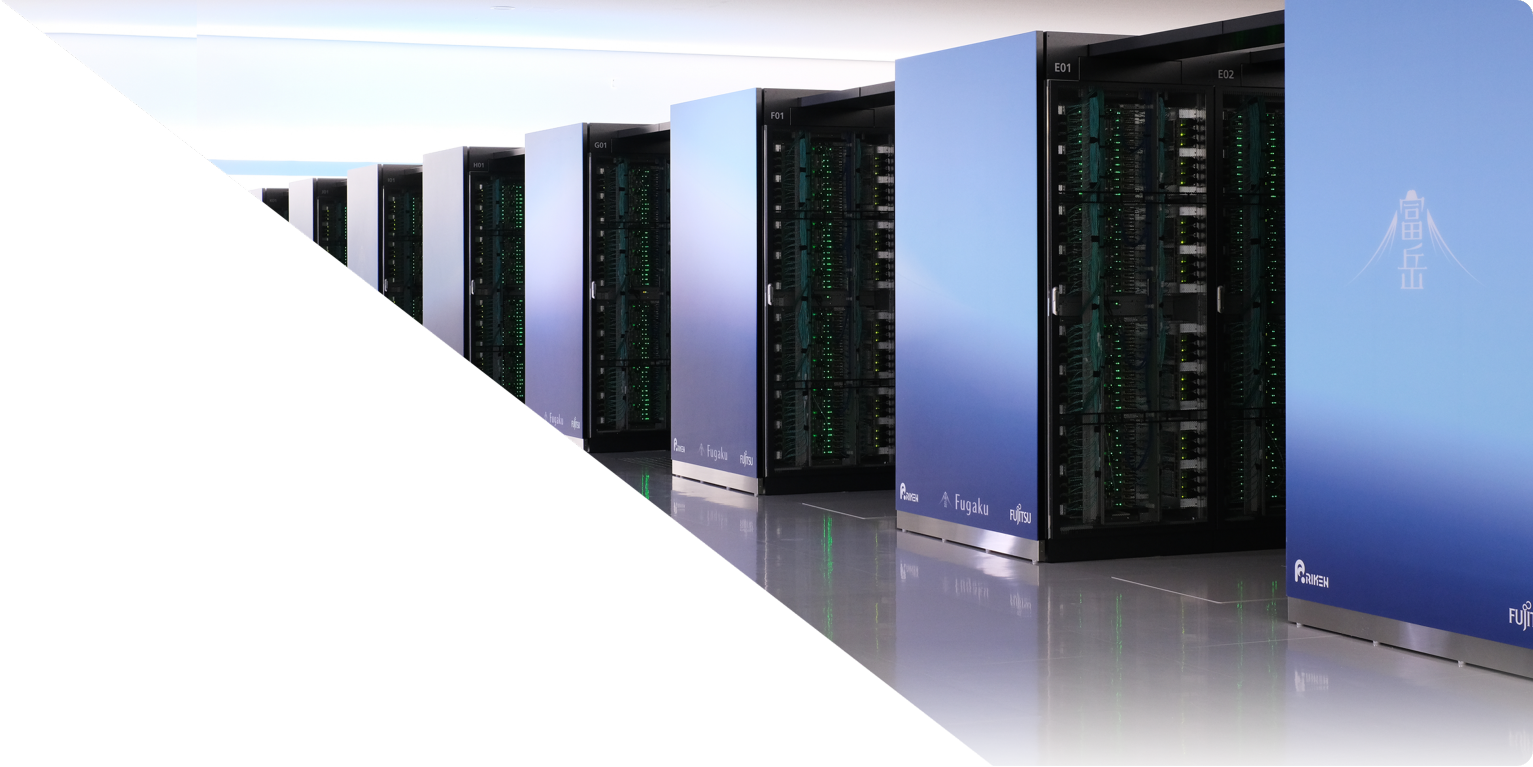
\includegraphics[width=0.7\paperwidth]{presentation/half-fugaku-bg}};
\node[rectangle, fill=white, path fading=fade right, minimum width=0.6\paperwidth, minimum height=1.5cm] (box) at (10cm,-1.6cm){};
\node[rectangle, fill=white, path fading=fade right, minimum width=0.6\paperwidth, minimum height=0.7cm] (box) at (10cm,-3.2cm){};
\node[above right,inner sep=0pt](wave) at (current page.south west) {
\includegraphics[scale=0.7]{presentation/wave1}};
\node[above right,inner sep=0pt](wave) at (wave.south east) {
\includegraphics[scale=0.5]{presentation/wave2}};
\end{tikzpicture}}{}
} %ifdraft
\setbeamercolor*{title}{use=structure}
\setbeamercolor{math text}{fg=structure.fg}
\usepackage{concmath, subcaption, qrcode}
\usepackage{tikz}
\usepackage{marvosym}
\usepackage[marvosym]{tikzsymbols}
\usetikzlibrary{arrows, matrix, arrows.meta, shapes, shapes.arrows, shapes.multipart, shapes.symbols, fadings, fit, positioning, decorations.pathreplacing, angles, quotes}
\setbeamercovered{transparent}
\usefonttheme{serif}
\usetheme{default}
\author{\alert{E. Vatai}, A. Drozd, I. R. Ivanov, Y. Ren, M. Wahib}
\date{\url{http://vatai.github.io/}}
\title{Enabling AI-based Automated Code Generation with Guaranteed Correctness}
\hypersetup{
 pdfauthor={\alert{E. Vatai}, A. Drozd, I. R. Ivanov, Y. Ren, M. Wahib},
 pdftitle={Enabling AI-based Automated Code Generation with Guaranteed Correctness},
 pdfkeywords={},
 pdfsubject={},
 pdfcreator={Emacs 29.4 (Org mode 9.7.11)}, 
 pdflang={English}}
\begin{document}

\maketitle
\section{Tadashi}
\label{sec:org6f39c4c}
\begin{frame}[label={sec:orgf9dc1c3}]{ML approaches to correctness in code generation}
\begin{columns}
\begin{column}{0.45\columnwidth}
\begin{itemize}
\item <1-> Extensive unit testing
\begin{itemize}
\item Coverage
\item Writing tests is not trivial
\end{itemize}
\item <3-> Surrogate ML model
\begin{itemize}
\item Trust issues
\end{itemize}
\item <4-> Limit ML to short sequences of instructions
\item <4-> Limit ML to a set of determined transformations
\begin{itemize}
\item Not general
\end{itemize}
\item <5-> Symbolic execution
\begin{itemize}
\item Not well established
\end{itemize}
\item <6-> Round-trip
\begin{itemize}
\item Trust issues
\end{itemize}
\end{itemize}
\end{column}
\begin{column}{0.45\columnwidth}
\begin{block}<2->{Edsger W. Dijkstra}
\begin{quote}
``Program testing can be used to show the presence of bugs, but never to show their absence!''
\end{quote}
\end{block}
\end{column}
\end{columns}
\end{frame}
\begin{frame}[label={sec:orgdb69c7f}]{}
\begin{center}

\includegraphics[width=0.5\textwidth]{./figs/xkcd.png}
\end{center}
\end{frame}
\begin{frame}[label={sec:org35fc1b0}]{All you need is to sample the set of correct transformations}
\begin{itemize}
\item <+-> \alert{ML codegen is transformations} on a reference implementation
\item <+-> ML can \alert{explore the space of transformations} to find a faster version
\item <+-> But we also need \alert{correctness}
\end{itemize}
\end{frame}
\begin{frame}[label={sec:org7790027}]{TADASHI: \alert{loop transformations} with correctness check}
\begin{center}
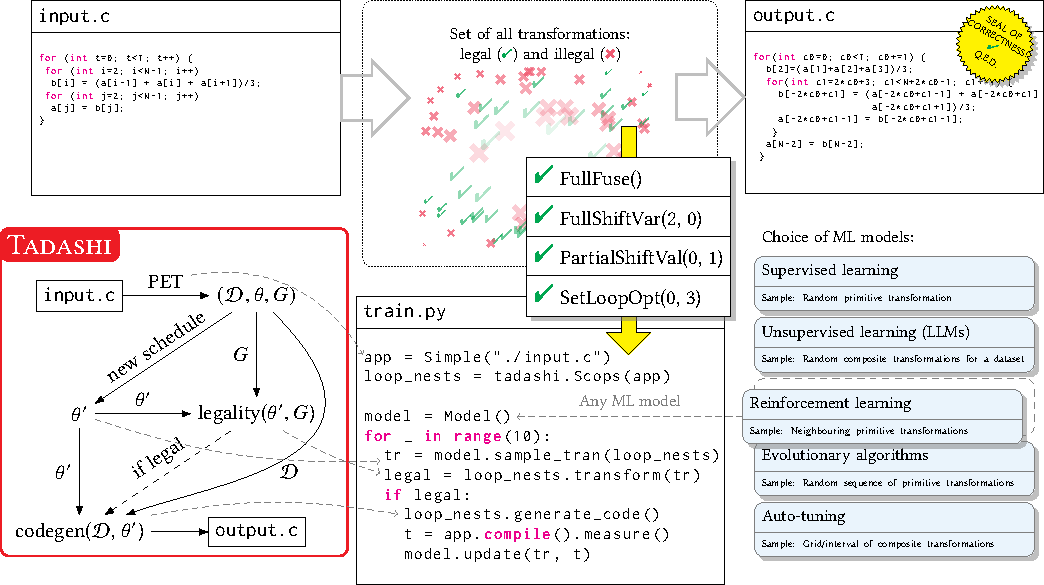
\includegraphics[width=.9\linewidth]{./figs/sampling.pdf}
\end{center}
\end{frame}
\begin{frame}[label={sec:orgd4bb48c}]{Reinforcement learning}
\begin{itemize}
\item Actions = primitive transformations; Reward = walltime; Environment = correctness
\end{itemize}
\begin{center}
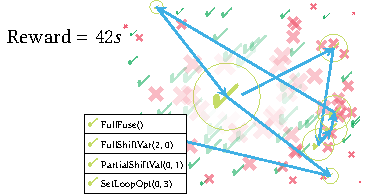
\includegraphics[width=0.7\textwidth]{./figs/ml-rl.pdf}
\end{center}
\end{frame}
\begin{frame}[label={sec:org921dcb3}]{Supervised learning}
\begin{itemize}
\item Dataset generation (legal transformations); Sample label: runtime
\end{itemize}
\begin{center}
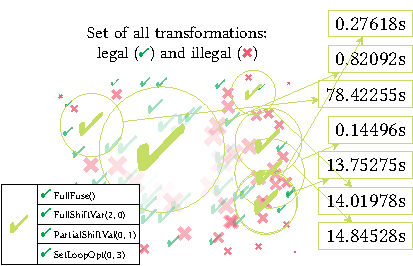
\includegraphics[width=0.7\textwidth]{./figs/ml-sl.pdf}
\end{center}
\end{frame}
\begin{frame}[label={sec:orgb938ab6}]{Evolutionary algorithms}
\begin{itemize}
\item Exploration and explorations; Candidates = transformations; Objective function = runtime
\end{itemize}
\begin{center}
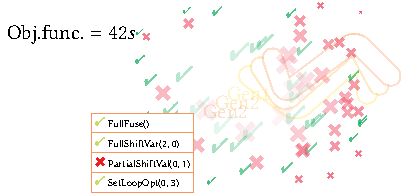
\includegraphics[width=0.7\textwidth]{./figs/ml-ea.pdf}
\end{center}
\end{frame}
\begin{frame}[label={sec:org78ea039}]{LLM agents}
\begin{itemize}
\item Dataset generation; High quality correct transformations; Caveat! Hallucinations are possible!
\end{itemize}
\begin{center}
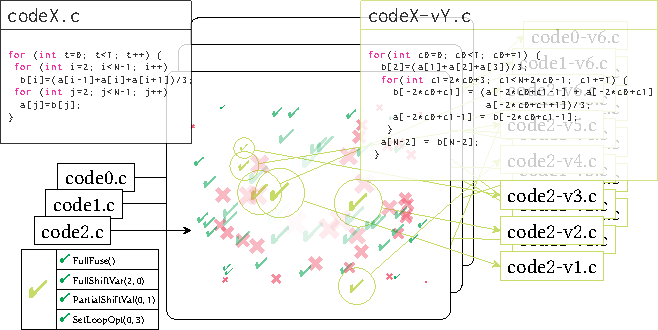
\includegraphics[width=0.8\textwidth]{./figs/ml-ul.pdf}
\end{center}
\end{frame}
\begin{frame}[label={sec:orgc6cfe5b}]{Auto-Tuning}
\begin{itemize}
\item Brute forcing on a bounded region of the space (grid search)
\end{itemize}
\begin{center}
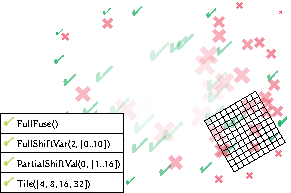
\includegraphics[width=0.7\textwidth]{./figs/ml-at.pdf}
\end{center}
\end{frame}
\begin{frame}[label={sec:org6dab10a}]{Grand vision}
\begin{block}{Large scale optimisation framework}
\begin{center}
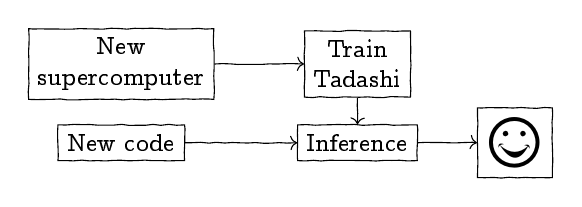
\begin{tikzpicture}[
  decoration={random steps,segment length=1mm,amplitude=0.2pt},
  every node/.style={decorate, draw}, align=center, font=\small,
  every edge/.style={draw, ->, decorate},
]
\node (new) {New\\supercomputer};
\node [right of=new, node distance=3cm] (train) {Train\\Tadashi};
\node [below of=new] (newcode) {New code};
\node [below of=train] (infer) {Inference};
\node [right of=infer, node distance=2cm] (done) {\Huge \Smiley};
\path
(new) edge (train)
(newcode) edge (infer)
(train) edge (infer)
(infer) edge (done);
\end{tikzpicture}
\end{center}
\end{block}
\begin{block}{Wise words}
\begin{quote}
Spending 6h on the whole machine to make the code 5\% faster will pay off.  -- N. D.
\end{quote}
\end{block}
\end{frame}
\begin{frame}[label={sec:org351ec09},fragile]{Now: Support C, Harness, and Transformations}
 \begin{center}
\begin{tabular}{ll}
\texttt{TrEnum} & Args\\
\hline
\texttt{TILE} & tile size\\
\texttt{INTERCHANGE} & --\\
\texttt{FULL\_FUSE} & --\\
\texttt{FUSE} & 2 loop indices\\
\texttt{FULL\_SHIFT\_VAL} & const shift value\\
\texttt{PARTIAL\_SHIFT\_VAL} & stmt idx, const shift value\\
\texttt{FULL\_SHIFT\_VAR} & coeff, shift iter idx\\
\texttt{PARTIAL\_SHIFT\_VAR} & stmt idx, coeff, shift iter idx\\
\texttt{FULL\_SHIFT\_PARAM} & coeff, shift param idx\\
\texttt{PARTIAL\_SHIFT\_PARAM} & stmt idx, coeff, shift param idx\\
\texttt{SCALE} & coeff\\
\texttt{SET\_PARALLEL} & --\\
\texttt{SET\_LOOP\_OPT} & \texttt{AstLoopType} enum\\
\end{tabular}
\end{center}
\end{frame}
\begin{frame}[label={sec:org0cd5127}]{Future:}
\begin{columns}
\begin{column}{0.48\columnwidth}
\begin{itemize}
\item New language
\begin{itemize}
\item Fortran (MLIR, Polygeist)
\item CUDA (PPCG?)
\end{itemize}
\item Better use of the polyhedral model
\begin{itemize}
\item New transformations: Loop fission, unrolling, etc.
\item Expansion and extension nodes
\item More efficient legality check
\end{itemize}
\end{itemize}
\end{column}
\begin{column}{0.48\columnwidth}
\begin{itemize}
\item Harness/infrastructure
\begin{itemize}
\item Scheduler support (slurm, pjsub)
\item Compiler flags
\end{itemize}
\item ML (target list)
\begin{itemize}
\item Reinforcement Learning
\item LLM Agents
\item Auto-Tuning
\item Supervised Learning
\item Evolutionary Algorithms
\end{itemize}
\end{itemize}
\end{column}
\end{columns}
\end{frame}
\begin{frame}[label={sec:org55d3329},fragile]{Random RL}
 \begin{minted}[]{python}
def train_model(app, num_iter=3, net=Model()):
  loop_nests = LoopNests(app)
  ln = loop_nests[0]
  for i in range(num_iter):
    loop_idx, tr, args = net.transform(ln)
    loop = ln.schedule_tree[loop_idx]
    legal = loop.transform(tr, *args)
    if not legal:
      node.rollback()
      continue
    loop_nests.generate_code("output.c")
    app.compile()
    t = app.measure()
    # net.update(loop_idx, tr, args, legal, t)
\end{minted}
\end{frame}
\begin{frame}[label={sec:org6d65bd2}]{Breakdown (primitive)}
\begin{center}
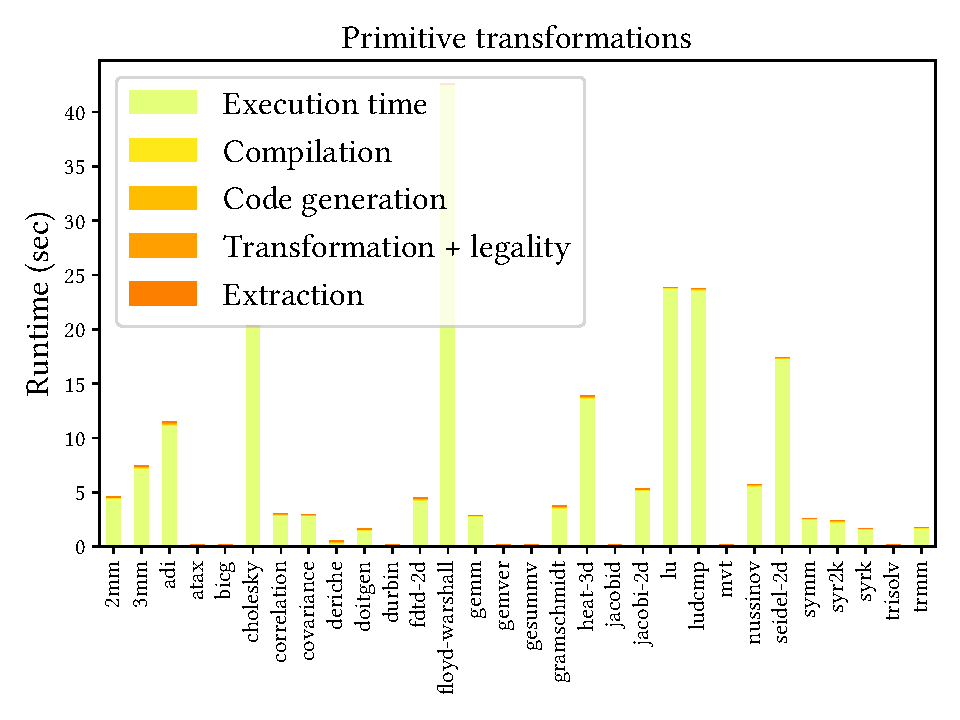
\includegraphics[width=0.7\textwidth]{./figs/plot-breakdown-abs-1.pdf}
\end{center}
\end{frame}
\begin{frame}[label={sec:org9e6c436}]{Breakdown (10 seq)}
\begin{center}
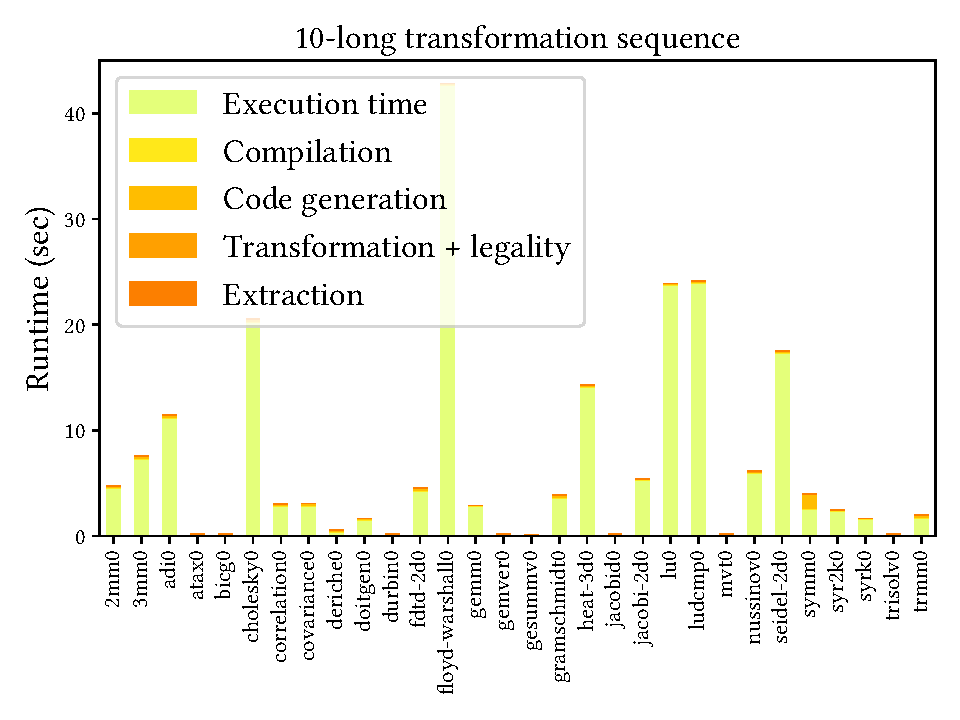
\includegraphics[width=0.7\textwidth]{./figs/plot-breakdown-abs-10.pdf}
\end{center}
\end{frame}
\begin{frame}[label={sec:orgb9bee36}]{Throughput}
\begin{center}
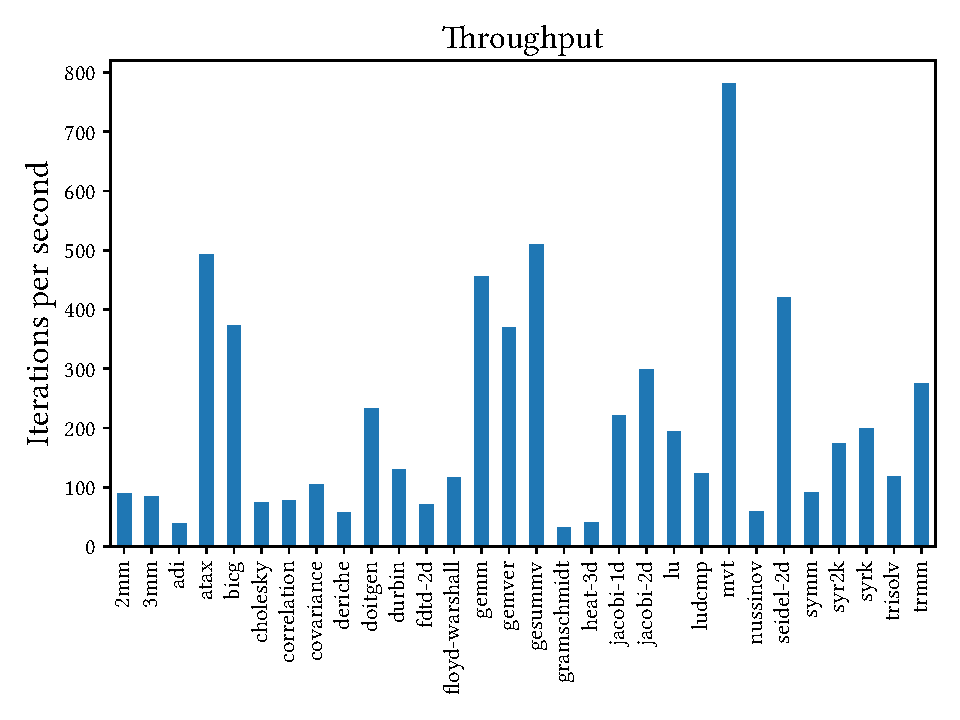
\includegraphics[width=0.7\textwidth]{./figs/plot-throughput.pdf}
\end{center}
\end{frame}
\begin{frame}[label={sec:orgdee6bbb}]{Representations}
Different levels of abstraction
\begin{itemize}
\item source code [Stein: Paraphrasing etc.]
\item abstract syntax tree (AST) [Shido: Tree-LSTM etc.]
\item polyhedral [Baghdadi: Tiramisu]
\item dependency graphs [Cummins: ProGraML]
\item intermediate Representations (IR) [Ben-nun: inst2vec]
\item assembly instructions [Deepmind: Faster sorting]
\end{itemize}
\end{frame}
\begin{frame}[label={sec:orgc5d72af},fragile]{Polyhedral model}
 \begin{columns}
\begin{column}{0.45\columnwidth}
\begin{block}{Components}
\begin{enumerate}
\item \(\mathcal{D}_S = \{ S[\vec{i}] \in \mathbb{Z}^n : \mathbf{A} \vec{i} + \mathbf{b} \le \mathbf{0}  \}\)
\item \(\theta(S[i, j]) = t = (i, j)\)
\item \(G=(V, E)\):
\begin{itemize}
\item \(V=\{ S_0, S_1, \ldots\}\),
\item \(E=\{ S_i[\vec{d}] \mapsto S_j[\vec{r}], \ldots \}\)
\end{itemize}
\end{enumerate}
\end{block}
\end{column}
\begin{column}{0.45\columnwidth}
\begin{block}{Mini example}
\begin{minted}[]{c}
for(int i = 0; i < N; i++)
  for(int j = 1; j < M; j++)
    A[i, j] += A[i, j-1]; // S[i,j]
\end{minted}
\end{block}
\end{column}
\end{columns}
\end{frame}
\begin{frame}[label={sec:orge1560a3}]{}
\begin{columns}
\begin{column}{0.45\columnwidth}
\begin{figure}
  \centering
  \subcaptionbox{$\theta(S[i, j]) = (i, j)$  \label{sf:schedule-i-j}}
  {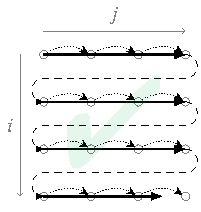
\includegraphics[width=0.48\linewidth]{figs/schedule-i-j}}
  \subcaptionbox{$\theta(S[i, j]) = (j, i)$  \label{sf:schedule-j-i}}
  {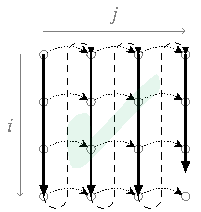
\includegraphics[width=0.48\linewidth]{figs/schedule-j-i}}
  \subcaptionbox{$\theta(S[i, j]) = (i+j, j)$\label{sf:schedule-ipj-j}}
  {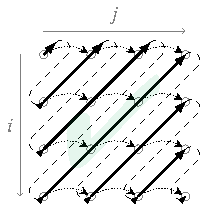
\includegraphics[width=0.48\linewidth]{figs/schedule-ipj-j}}
  \subcaptionbox{$\theta(S[i, j]) = (i, -j)$ \label{sf:schedule-i-mj}}
  {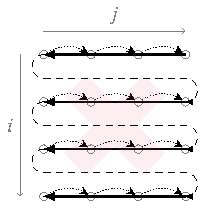
\includegraphics[width=0.48\linewidth]{figs/schedule-i-mj}}
  \label{fig:schedules}
\end{figure}
\end{column}
\begin{column}{0.52\columnwidth}
\begin{block}{Legality check}
\begin{center}
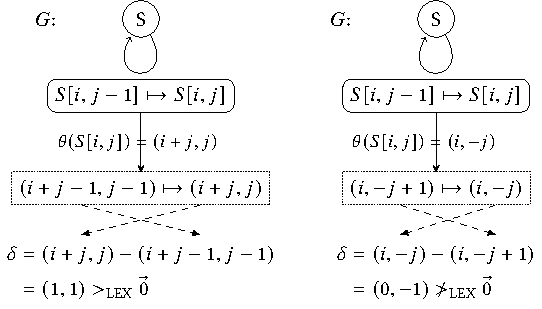
\includegraphics[width=\linewidth]{./figs/legality.pdf}
\end{center}
\end{block}
\end{column}
\end{columns}
\end{frame}
\begin{frame}[label={sec:org3da4216},fragile]{End-to-end example}
 \begin{minted}[]{python}
import tadashi
app = tadahis.Simple("input.c")
scops = tadahi.Scops(app)
node = scops[0].schedule_tree[1]
tr, args = tadashi.TrEnum.TILE, 16
legal = node.transform(tr, args)
if legal:
    scops.generate_code(output_path="output.c")
    app.compile()
    t = app.measure()
    printf(f"Walltime: {t}")
\end{minted}
\end{frame}
\begin{frame}[label={sec:orgd726f4c}]{}
\begin{center}
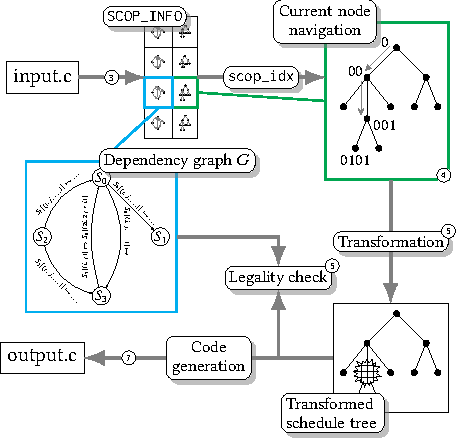
\includegraphics[width=0.65\textwidth]{./figs/design.pdf}
\end{center}
\end{frame}
\begin{frame}[label={sec:org06b8dce}]{That's all folks!}
\begin{itemize}
\item i. \url{https://vatai.github.io/}
\item ii. \url{https://github.com/vatai/tadashi/}
\item iii. \url{https://arxiv.org/abs/2410.03210}
\end{itemize}

\bigskip

i. \qrcode{https://vatai.github.io/} \hfill
ii. \qrcode{https://github.com/vatai/tadashi/} \hfill
iii. \qrcode{https://arxiv.org/abs/2410.03210}
\end{frame}
\end{document}
